\let\lesson\undefined
\newcommand{\lesson}{\phantomlesson{Bài 4: Nhiệt dung riêng, nhiệt nóng chảy riêng, nhiệt hoá hơi riêng}}
\chapter[Bài tập về sự chuyển thể]{Bài tập về sự chuyển thể}
\section{Ôn tập lý thuyết}
\subsection{Nhiệt lượng trao đổi để vật thay đổi nhiệt độ (không có sự chuyển thể)}
\begin{equation}
	Q=mc\Delta t=mc\left(t_2-t_1\right)
\end{equation}
với:
\begin{itemize}
	\item $Q$: nhiệt lượng trao đổi, đơn vị trong hệ SI là $\si{\joule}$;
	\item $m$: khối lượng của khối chất, đơn vị trong hệ SI là $\si{\kilogram}$;
	\item $c$: nhiệt dung riêng của khối chất, đơn vị trong hệ SI là $\si{\joule/\left(\kilogram\cdot\kelvin\right)}$;
	\item $\Delta t=t_2-t_1$: độ biến thiên nhiệt độ của vật, đơn vị trong hệ SI là $\si{\kelvin}$.
\end{itemize}
\subsection{Sự chuyển thể của các chất}
\begin{center}
	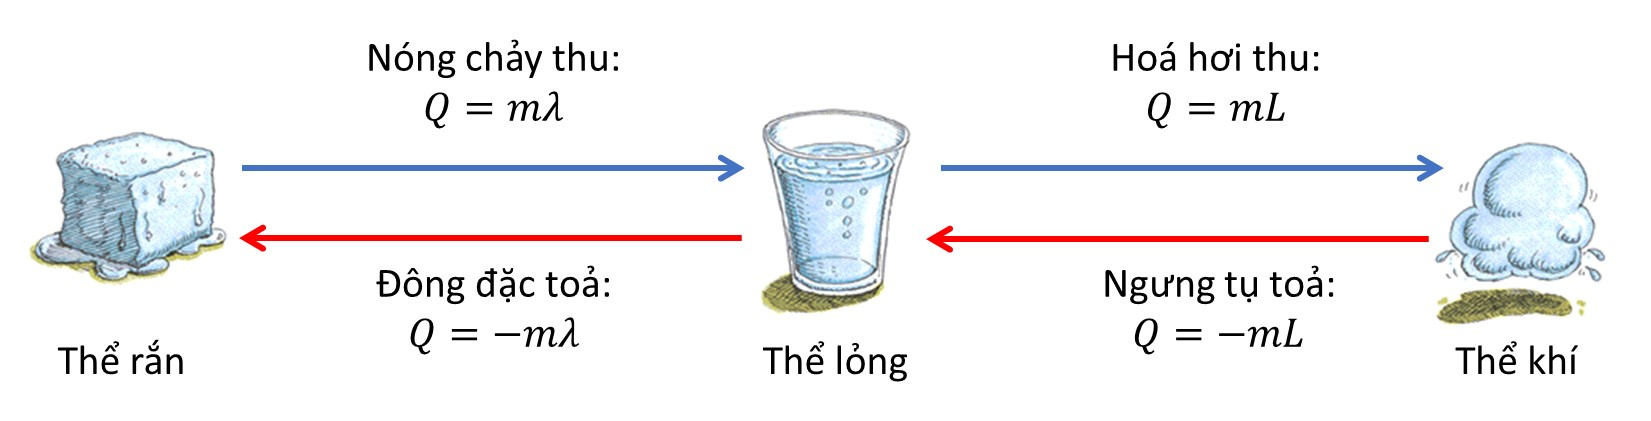
\includegraphics[width=0.8\linewidth]{../figs/VN12-Y24-PH-SYL-006-1}
	\captionof{figure}{Sơ đồ chuyển thể}
\end{center}
\section{Mục tiêu bài học - Ví dụ minh hoạ}
\begin{dang}{Áp dụng phương trình cân bằng nhiệt khi có sự chuyển thể}
	\viduii{3}
	{Rót nước ở nhiệt độ $t_1=\SI{20}{\celsius}$ vào một nhiệt lượng kế. Thả vào trong nhiệt lượng kế một cục nước đá khối lượng $m_2=\SI{0.5}{\kilogram}$ và nhiệt độ $t_2=\SI{-15}{\celsius}$. Biết khối lượng nước đổ vào $m_1=m_2$. Cho biết nhiệt dung riêng của nước $c_1=\SI{4200}{\joule/\left(\kilogram\cdot\kelvin\right)}$, của nước đá $c_2=\SI{2100}{\joule/\left(\kilogram\cdot\kelvin\right)}$ và nhiệt nóng chảy riêng của nước đá $\lambda=\SI{3.4E5}{\joule/\kilogram}$. Bỏ qua sự trao đổi nhiệt với môi trường.
	\begin{enumerate}[label=\alph*)]
		\item Hãy cho biết cục nước đá có tan hết không?
		\item Nếu nước đá tan hết, hãy xác định nhiệt độ của hỗn hợp sau khi cân bằng nhiệt được thiết lập. Nếu nước đá không tan hết, hãy tính khối lượng nước đá đã tan.
	\end{enumerate}
}
{ \hide{\begin{enumerate}[label=\alph*)]
		\item Nhiệt lượng nước $\SI{20}{\celsius}$ toả ra để giảm nhiệt độ xuống $\SI{0}{\celsius}$:
		$$Q_1=m_1c_1\left(0-t_1\right)=\left(\SI{0.5}{\kilogram}\right)\cdot\left[\SI{4200}{\joule/\left(\kilogram\cdot\kelvin\right)}\right]\cdot\left(\SI{0}{\celsius}-\SI{20}{\celsius}\right)=\SI{-42000}{\joule}.$$
		Nhiệt lượng nước đá cần thu vào để tăng nhiệt độ từ $\SI{-15}{\celsius}$ đến $\SI{0}{\celsius}$ và nóng chảy hoàn toàn:
		$$Q_2=m_2c_2\left(0-t_2\right)+m_2\lambda$$
		$$\Leftrightarrow Q_2=\left(\SI{0.5}{\kilogram}\right)\cdot\left[\SI{2100}{\joule/\left(\kilogram\cdot\kelvin\right)}\right]\cdot\left(\SI{0}{\celsius}+\SI{15}{\celsius}\right)+\left(\SI{0.5}{\kilogram}\right)\cdot\left(\SI{3.4E5}{\joule/\kilogram}\right)=\SI{185750}{\joule}.$$
		Vì $\left|Q_1\right|<Q_2$ nên nước đá chỉ tan được một phần.
		\item Vì nước đá chỉ tan một phần nên nhiệt độ của hỗn hợp khi cân bằng nhiệt là $\SI{0}{\celsius}$.\\
		Gọi $m'$ là khối lượng nước đá đã tan.\\
		Nhiệt lượng nước đá cần thu vào để tăng nhiệt độ từ $\SI{-15}{\celsius}$ đến $\SI{0}{\celsius}$ và nóng chảy một phần: $$Q_2'=m_2c_2\left(0-t_2\right)+m'\lambda.$$
		Trạng thái cân bằng nhiệt được thiết lập khi tổng nhiệt lượng trao đổi trong hệ bằng 0:
		$$Q_1+Q_2'=0$$
		$$\Leftrightarrow Q_1+m_2c_2\left(0-t_2\right)+m'\lambda=0$$
		\begin{eqnarray*}
			\Rightarrow m'&=&-\dfrac{Q_1+m_2c_2\left(0-t_2\right)}{\lambda}\\
			\Leftrightarrow m'&=&-\dfrac{\SI{-42000}{\joule}+\left(\SI{0.5}{\kilogram}\right)\cdot\left[\SI{2100}{\joule/\left(\kilogram\cdot\kelvin\right)}\right]\cdot\left(\SI{0}{\celsius}+\SI{15}{\celsius}\right)}{\SI{3.4E5}{\joule/\kilogram}}\\
			\Rightarrow m'&\approx&\SI{77.2}{\gram}.
		\end{eqnarray*}
	Vậy khối lượng nước đá đã tan là $\SI{77.2}{\gram}$.
	
		
	\end{enumerate}}
}

\viduii{3}
{Dẫn $m_1=\SI{100}{\gram}$ hơi nước ở $t_1=\SI{100}{\celsius}$ vào một bình cách nhiệt đựng nước đá ở $t_2=\SI{-4}{\celsius}$. Nước đá bị tan hoàn toàn và nhiệt độ nước trong bình sau khi cân bằng nhiệt là $\SI{10}{\celsius}$. Tìm khối lượng nước đá trong bình. Biết nhiệt nóng chảy riêng của nước đá là $\lambda=\SI{3.4E5}{\joule/\kilogram}$, nhiệt hoá hơi riêng của nước ở $\SI{100}{\celsius}$ là $L=\SI{2.3E6}{\joule/\kilogram}$, nhiệt dung riêng của nước là $c_1=\SI{4200}{\joule/\left(\kilogram\cdot\kelvin\right)}$, nhiệt dung riêng của nước đá là $c_2=\SI{2100}{\joule/\left(\kilogram\cdot\kelvin\right)}$. Bỏ qua sự trao đổi nhiệt với môi trường.

}
{\hide{Gọi $\xsi{m}{\left(\kilogram\right)}$ là khối lượng nước đá trong bình.\\
	Nhiệt lượng hơi nước toả ra để ngưng tụ hoàn toàn ở $\SI{100}{\celsius}$ và giảm nhiệt độ từ $\SI{100}{\celsius}$ xuống $\SI{10}{\celsius}$:
	$$Q_1=-m_1L+m_1c_1\left(t_\text{cb}-t_1\right)$$
	$$\Leftrightarrow Q_1=-\left(\SI{0.1}{\kilogram}\right)\cdot\left(\SI{2.3E6}{\joule/\kilogram}\right)+\left(\SI{0.1}{\kilogram}\right)\cdot\left[\SI{4200}{\joule/\left(\kilogram\cdot\kelvin\right)}\right]\cdot\left(\SI{10}{\celsius}-\SI{100}{\celsius}\right)=\SI{-267800}{\joule}.$$
	Nhiệt lượng nước đá thu vào để tăng nhiệt độ từ $\SI{-4}{\celsius}$ lên $\SI{0}{\celsius}$, nóng chảy hoàn toàn ở $\SI{0}{\celsius}$ rồi tăng nhiệt độ lên $\SI{10}{\celsius}$:
	$$Q_2=mc_2\left(0-t_2\right)+m\lambda+mc_1\left(t_\text{cb}-0\right)$$
	$$\Leftrightarrow Q_2=m\cdot\left[\SI{2100}{\joule/\left(\kilogram\cdot\kelvin\right)}\right]\cdot\left(\SI{0}{\celsius}+\SI{4}{\celsius}\right)+m\cdot\left(\SI{3.4E5}{\joule/\kilogram}\right)+m\cdot\left[\SI{4200}{\joule/\left(\joule\cdot\kelvin\right)}\right]\cdot\left(\SI{10}{\celsius}-\SI{0}{\celsius}\right)=390400m.$$
	Hệ đạt trạng thái cân bằng nhiệt khi tổng nhiệt lượng trao đổi trong hệ bằng 0:
	\begin{eqnarray*}
		&&Q_1+Q_2=0\\
		&\Leftrightarrow& -267800+390400m=0\\
		&\Rightarrow& m\approx\SI{0.686}{\kilogram}.
	\end{eqnarray*}
}
}
	
\end{dang}